\documentclass[11pt]{article}

\usepackage{amsmath}
\usepackage{textcomp}
\usepackage[top=1in, bottom=1in, left=1.2in, right=1.2in]{geometry}

% Add other packages here %
\usepackage{indentfirst}
\usepackage{float}
\usepackage[usenames, dvipsnames]{color}
\usepackage{graphicx}
\graphicspath{ {./images/} }
\renewcommand{\labelitemi}{\textendash}

% Put your group number and names in the author field %
\title{\bf Exercise 4\\ Implementing a centralized agent}
\author{Group \textnumero:44 Valentin Kindschi, Cyril van Schreven}


% N.B.: The report should not be longer than 3 pages %


\begin{document}
\maketitle

\section{Solution Representation}

Our implementation of a centralized agent is inspired by the document "Finding the Optimal Delivery Plan"\footnote{\textit{"Finding the Optimal Delivery Plan:Model as a Constraint Satisfaction Problem"}. Radu Jurca, Nguyen Quang Huy and Michael Schumacher}. To allow vehicles to carry multiple tasks, we split the elementary unit of a task into two actions: the action of picking up and the action of delivering. The algorithms and constraints are updated accordingly.

\subsection{Variables}
% Describe the variables used in your solution representation %
We used four different map objects in our solution: $nextActionA$ mapping action to action, $nextActionV$ mapping action to vehicle, $time$ mapping action to integer, $vehicle$ mapping action to vehicle.

\subsection{Constraints}
% Describe the constraints in your solution representation %
The same constraints as in the above mentioned document are used. The constraint regarding capacity has been changed to verify the available capacity after each action. An extra constraint has been added to force a delivery action to be later than a pickup action


\subsection{Objective function}
% Describe the function that you optimize %
The objective function is the sum of the cost of each vehicle. The cost is computed as the $costPerKm*totalDistance$.

We explored a second objective function. The aim is to accomplish all the tasks as quickly as possible. For this the objective function is the cost of the vehicle with the highest cost.


\section{Stochastic optimization}

\subsection{Initial solution}
% Describe how you generate the initial solution %
For the initial solution, all the tasks are assigned to the vehicle with the largest carrying capacity. It delivers all the tasks sequentially without carrying multiple tasks. An error is triggered if a task is heavier than its total capacity.

\subsection{Generating neighbours}
% Describe how you generate neighbors %
To generate neighbours, first a random vehicle with a task to perform is chosen. Then, the function $changingVehicle()$ gives the first task of the chosen vehicle to all the other vehicles, which will create a new neighbour plan per vehicle. A second function $changingActionOrder()$ will affect the order of the task handled by the same chosen vehicle. All possible permutations will create a new plan.
In the end, at most: 
$$ (\#Vehicles-1) + \#Tasks_{RandomVehicle} \cdot (\#Tasks_{RandomVehicle}-1)/2 $$ neighbours solution are computed for each iteration from which all the solution that do not meet the constraints are removed.


\subsection{Stochastic optimization algorithm}
% Describe your stochastic optimization algorithm %
Our stochastic algorithm will select the solution that minimizes the objective function between all the generated neighbour solution. There is also a probability $probAddCurrent$ that the current best solution, i.e. the previous best plan, is added to the possible solutions. This means that the previous solution is not automatically reelected if its neighbours solution are worst, which increased the exploration and allow to avoid local minimas. 
We also added a probability $probPickRandom$ that a random neighbour solution is chosen instead of the optimal one. This probability has an initial value which will decrease linearly with the iteration number to have more exploration in the beginning of the optimization.
Finally, we added a $Dropout$ parameter that was ignoring a proportion of the neighborood for the selection.

\section{Results}

\subsection{Experiment 1: Model parameters}
% if your model has parameters, perform an experiment and analyze the results for different parameter values %
In the first experiment, the two parameters were the probability $probAddCurrent$ to add the previous best solution to the pool of possible solutions and the objective function. The topology used was England.

\subsubsection{Setting}
% Describe the settings of your experiment: topology, task configuration, number of tasks, number of vehicles, etc. %
% and the parameters you are analyzing %

\begin{table}[H]
\centering
\begin{tabular}{|l|c||l|c|}
\hline
\textbf{Iterations}         & 5000      & \textbf{Number of Tasks}      & 30      \\ \hline
\textbf{$probAddCurrent$}   & Variable  & \textbf{Number of Vehicles}   & 4       \\ \hline
\textbf{$Dropout$} & Variable & \textbf{Vehicle's capacities} & 9       \\ \hline
\textbf{$probPickRandom_0$}   & 0.5  & \textbf{Objective function}             & Sum / Max \\ \hline
\end{tabular}
\caption{Setting experiment 1}
\end{table}

\subsubsection{Observations}
% Describe the experimental results and the conclusions you inferred from these results %

\begin{figure}[H]
	\centering
	\begin{minipage}{0.49\linewidth}
    	\centering
    	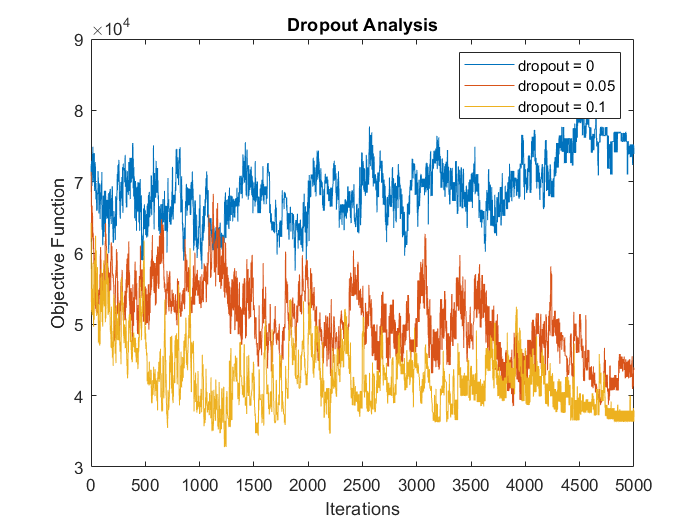
\includegraphics[scale = 0.45]{centralized/img/dropout.png}
    	\caption{Dropout Analysis}
        \label{fig:dropout}
	\end{minipage}
	\begin{minipage}{0.49\linewidth}
    	\centering
    	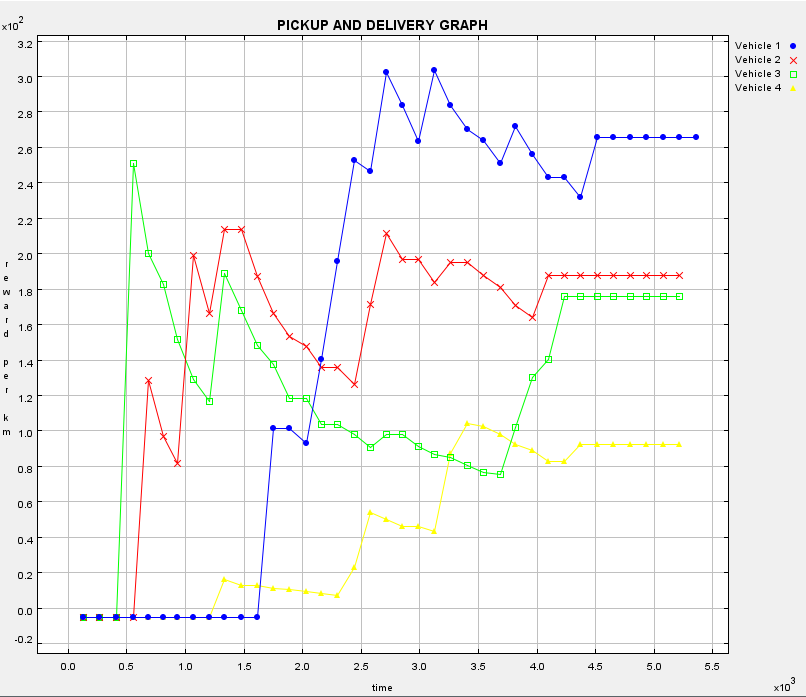
\includegraphics[scale = 0.42]{centralized/img/max.PNG}
    	\caption{Max Objective Function Results}
        \label{fig:max}
	\end{minipage}
\end{figure}

As we can see on Figure \ref{fig:dropout}, the dropout decreases the objective function values between 0 and 0.1, after which its impact becomes negligible. We also tried to vary $probAddCurrent$ between 0 and 1 and we did not notice any change in the objective function results. This is probably due to the fact that we add a lot of stochasticity in our algorithm and including the previous best solution does not really impact the results.

On Figure \ref{fig:max} one can see that using a Max objective function instead of using the sum over all the vehicles, the work is well distributed between and the tasks are all achieved a lot quicker. In fact, with the sum function a single agent is carrying most of the tasks which takes more time, but reduces the total cost between all the vehicles.

\subsection{Experiment 2: Different configurations}
% Run simulations for different configurations of the environment (i.e. different tasks and number of vehicles) %

\subsubsection{Setting}
% Describe the settings of your experiment: topology, task configuration, number of tasks, number of vehicles, etc. %

In this experiment we try to observe the impact of varying the number of vehicles and the capacity. We kept the parameters as for the previous experiment and used a dropout of 0.1.

\subsubsection{Observations}
Varying the number of vehicles did not affect the results in a noticeable way. This highlights the fact that one single vehicle performs almost all the tasks.
\begin{table}[H]
\centering
\begin{tabular}{|l|c|c|c|c|}
\hline
\textbf{Capacity} & 1      & 2      & 3      & 4      \\ \hline
\textbf{Cost}   & 74'661 & 45'608 & 38'237 & 29'133 \\
       \hline
\end{tabular}
\caption{Capacity Analysis}
\end{table}
As expected with a higher capacity, the tasks can be delivered for a lesser cost. This shows that the algorithm is capable of properly arranging actions.




% Describe the experimental results and the conclusions you inferred from these results %
% Reflect on the fairness of the optimal plans. Observe that optimality requires some vehicles to do more work than others. %
% How does the complexity of your algorithm depend on the number of vehicles and various sizes of the task set? %

\end{document}